\documentclass[11pt,a4paper]{article}
\usepackage[margin=2cm]{geometry}
\usepackage{amsmath,graphicx,xcolor,caption}
\title{Lists, Colours and Figures}
\author{Technical Writing Practical}
\date{}
\definecolor{custommagenta}{RGB}{200,20,200}
\colorlet{redyellow}{red!60!yellow}
\begin{document}
\maketitle
\section{Lists}
Following are some technologies that can be used to format content:
\begin{itemize}
\item \LaTeX
\item HTML (+CSS)
\item Markdown
\end{itemize}
You would most likely use \LaTeX{} in the following scenarios:
\begin{enumerate}
\item To write research papers.
\item To embed mathematical equations within other software.
\item To create CVs, project reports and presentations.
\end{enumerate}
\section{Markup Types}
\begin{description}
\item[Presentational] Formatting embedded in text to produce a WYSIWYG result; example: Microsoft Word.
\item[Procedural] Markup provides instructions for programs to process text; example: \TeX.
\item[Descriptive] Labels parts of a document according to meaning; examples: \LaTeX{} and HTML5.
\end{description}
\section{Tables and Colours}
\begin{table}[!t]\centering
\caption{Example table with column widths}
\begin{tabular}{|p{3cm}|p{4cm}|p{3cm}|}\hline
\textbf{Column 1}&\textbf{Column 2}&\textbf{Column 3}\\\hline
First entry&Second entry&Third entry\\\hline
\multicolumn{3}{|c|}{Combined row across all columns}\\\hline
\end{tabular}
\end{table}
\[
\textcolor{custommagenta}{T(n)=aT(n/b)+f(n)}
\qquad
\textcolor{redyellow}{T(n)=aT(n/b)+f(n)}
\]
\section{Figures: Rotation and Cropping}
The course image files can be placed beside this source as \texttt{mnit-logo.png} and \texttt{mnit-building.jpg}.
\begin{figure}[ht]\centering
\IfFileExists{mnit-logo.png}
{
\includegraphics[angle=90,width=0.25\textwidth]{mnit-logo.png}}
{\fbox{\parbox[c][2cm][c]{0.25\textwidth}{\centering Add\\mnit-logo.png}}}
\caption{MNIT logo}
\end{figure}
\begin{figure}[ht]\centering
\IfFileExists{mnit-building.jpg}
{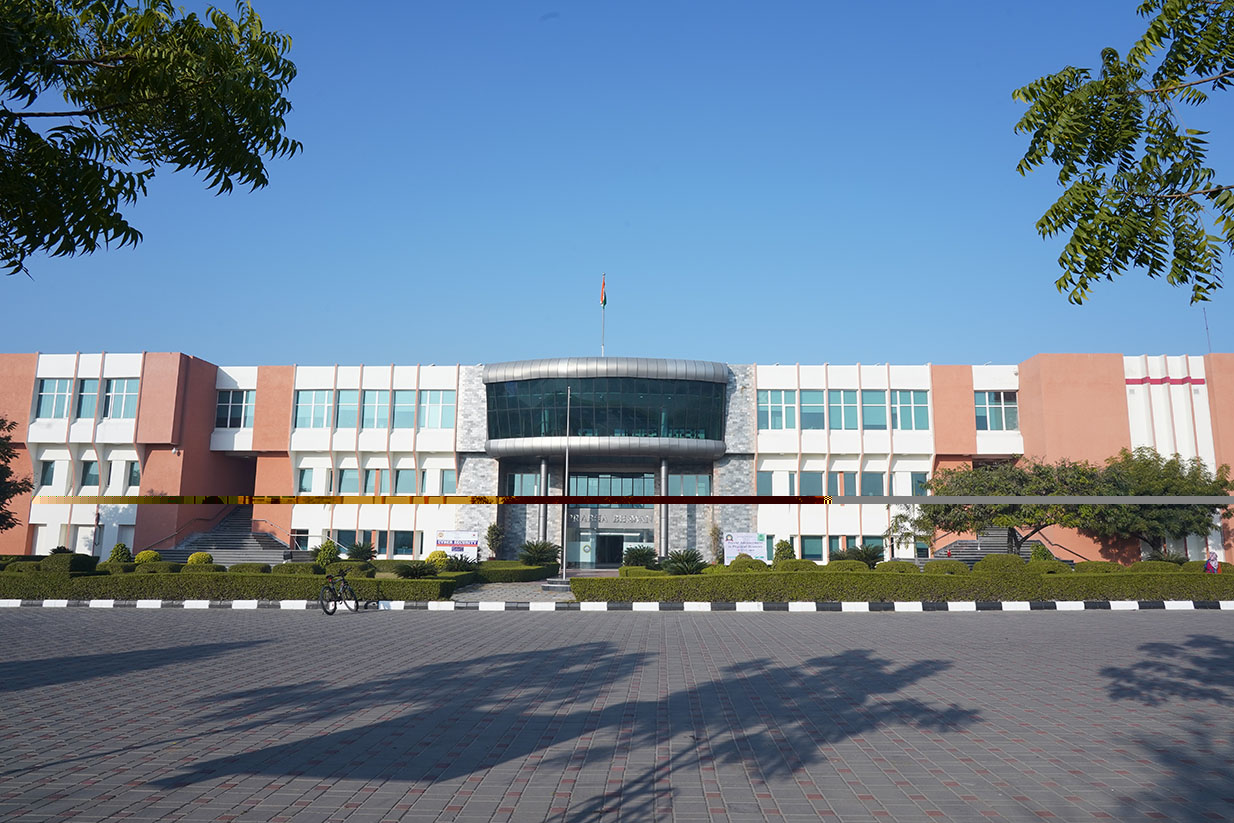
\includegraphics[width=\textwidth,trim=0 2cm 0 2cm,clip]{mnit-building.jpg}}
{\fbox{\parbox[c][3cm][c]{0.9\textwidth}{\centering Add mnit-building.jpg; crop sky with trim and clip.}}}
\caption{This is a floating image and can appear anywhere.}
\end{figure}
\section{Multiple Images Using Minipages}
\begin{figure}[ht]\centering
\begin{minipage}{0.45\textwidth}\centering
\fbox{\parbox[c][2cm][c]{0.9\linewidth}{\centering First image placeholder}}
\captionof{figure}{This is the first minipage}
\end{minipage}\hfill
\begin{minipage}{0.45\textwidth}\centering
\fbox{\parbox[c][2cm][c]{0.9\linewidth}{\centering Second image placeholder}}
\captionof{figure}{This is the second minipage}
\end{minipage}
\end{figure}
\end{document}
